% COLOURS.TEX
%
% The documentation in this file is part of PyXPlot
% <http://www.pyxplot.org.uk>
%
% Copyright (C) 2006-2010 Dominic Ford <coders@pyxplot.org.uk>
%               2008-2010 Ross Church
%
% $Id$
%
% PyXPlot is free software; you can redistribute it and/or modify it under the
% terms of the GNU General Public License as published by the Free Software
% Foundation; either version 2 of the License, or (at your option) any later
% version.
%
% You should have received a copy of the GNU General Public License along with
% PyXPlot; if not, write to the Free Software Foundation, Inc., 51 Franklin
% Street, Fifth Floor, Boston, MA  02110-1301, USA

% ----------------------------------------------------------------------------

% LaTeX source for the PyXPlot Users' Guide

\chapter{Colour Tables}
\label{ch:colour_charts}

\index{colours!charts} Figures~\ref{fig:colour_table1}, \ref{fig:colour_table2}
and \ref{fig:colour_table3} show the named colours which PyXPlot recognises.
These figures exclude the 100~shades of grey which PyXPlot recognises, which
are named from {\tt grey00} (black) to {\tt grey99} (almost white).  These
shades of grey may also be spelt {\tt gray??}.  \index{colours!shades of grey}

\begin{figure}
\begin{center}

\includegraphics[width=\textwidth]{figures/pyx_colours2}
\end{center}
\caption[A list of the named colours which PyXPlot recognises, sorted alphabetically]
{A list of the named colours which PyXPlot recognises, sorted alphabetically. The numerous shades of grey which it recognises are not shown.}
\label{fig:colour_table1}
\end{figure}

\begin{figure}
\begin{center}

\includegraphics[width=\textwidth]{figures/pyx_colours3}
\end{center}
\caption[A list of the named colours which PyXPlot recognises, sorted by hue]
{A list of the named colours which PyXPlot recognises, sorted by hue. The numerous shades of grey which it recognises are not shown.}
\label{fig:colour_table2}
\end{figure}

\begin{figure}
\begin{center}
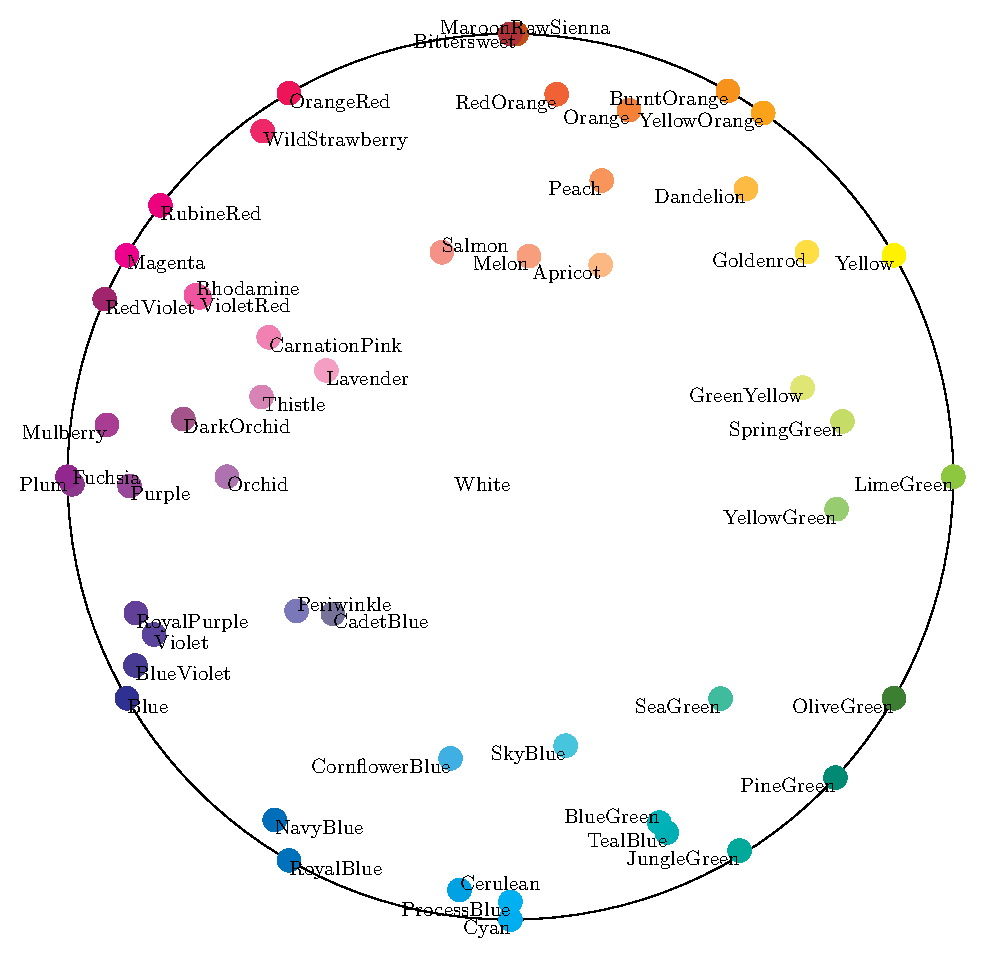
\includegraphics[width=\textwidth]{figures/pyx_colours}
\end{center}
\caption[The named colours which PyXPlot recognises, arranged in HSB colour space]
{The named colours which PyXPlot recognises, arranged in HSB colour space, with the brightness axis orientated into the page. Some colours are not shown as they lie too close to others.}
\label{fig:colour_table3}
\end{figure}

